%!TEX encoding = UTF-8 Unicode
\documentclass[12pt]{article} 
\usepackage[left=0.75in,top=20mm,right=0.75in,bottom=0.1in]{geometry} % Document margins
\usepackage{CJK}
\usepackage{graphicx}
\usepackage{mathtools}
\usepackage{mathrsfs}
\usepackage{amssymb}
\usepackage{hyperref}
\usepackage{sidecap}
\usepackage{makecell}
\usepackage{fancyhdr}

\fancypagestyle{title}{
 	\setlength{\headheight}{15pt}
	\fancyhf{}
	\renewcommand{\headrulewidth}{0pt}
	\renewcommand{\footrulewidth}{0pt}
	\fancyhead[R]{Parallel Programming 2015}
}

\pagestyle{title}

\makeatletter
\renewenvironment{itemize}
{\list{$\bullet$}{\leftmargin\z@ \labelwidth\z@ \itemindent-\leftmargin
\let\makelabel\descriptionlabel}}
{\endlist}
\makeatother

\begin{CJK}{UTF8}{bsmi}
\title{\textbf{Homework 1 / Odd-Even Sort}}
\author{\textbf{李豪韋 (HW-Lee) ID 103061527}}
\date{}

\begin{document}
\vspace*{-70pt}
{\let\newpage\relax\maketitle}
\thispagestyle{title}
\vspace*{-40pt}

\section*{Overview}
\vspace{-20pt}
\noindent\makebox[\linewidth]{\rule{\textwidth}{0.4pt}}
\vspace{-5pt}

There is a comparison sorting algorithm called \href{https://en.wikipedia.org/wiki/Odd\%E2\%80\%93even_sort}{odd-even sort}, which is also related to \href{https://en.wikipedia.org/wiki/Bubble_sort}{bubble sort}. It consists of two phases to sort a sequence, odd phase and even phase. At each iteration, the sequence will be separated into a couple of pairs, where the processor should arrange its to keep its in descending/ascending order. The process will keep running until there is no swapping in both even and odd phase. Due to independence among pairs, this algorithm can be accellerated with parallel implementations. In this project, the advantages of parallelism can be observed with different strategies.

\vspace{-5pt}
\section*{Implementation}
\vspace{-20pt}
\noindent\makebox[\linewidth]{\rule{\textwidth}{0.4pt}}

\begin{enumerate}
	\item Basic
	\begin{flushleft}
		The concept of the algorighm has been illustrated below, see Fig.1. After each processor has got its own data, only numbers at sides, i.e. at first or at end, have to be sent/received. Every processor swaps a pair of data if needed, and repeats the operation until there is no need to swap data.
	\end{flushleft}
	\item Advanced
	\begin{flushleft}
		The schema is similar to the basic version, the only difference is at the stage where each processor commences to re-arrange the sequence. After got the data, each processor will sort its sequence first. Then processors with rank $k$ will send the first number, which is the minimum (in ascending) or the maximum (in descending), to those with rank $k-1$, and then processors with rank $k-1$ will insert the received number and return back the last number, which is the maximum (in ascending) or the minimum (in descending). The operation will be executed until there is no change of all processors. In this project, there are two options chosen to be the pre-sorting algorithm, namely merge and bubble sort.
	\end{flushleft}
\end{enumerate}

\vspace{-23pt}
\begin{center}
	\begin{SCfigure}[][h]
		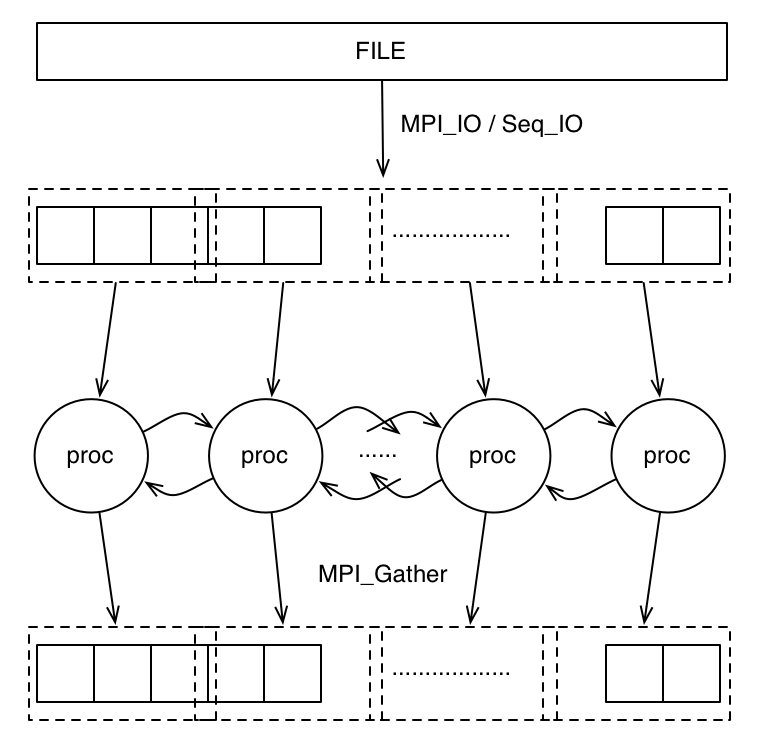
\includegraphics[scale=.27]{./overall_algo.png}
		\caption{Diagram of odd-even sort.
		\newline It mainly consists of 5 stages: 
		\newline 1) Input, to load data into registers.
		\newline 2) Scattering, to choose the fragment for which each processor should take responsibility. Each fragment will be sorted in advanced version. (with bubble/merge sort)
		\newline 3) Swapping at odd-even phase, core of the algorithm, iterates operation until there is no swapping occurred.
		\newline 4) Gathering, to merge all sorted data from processors.
		\newline 5) Output, to write the sorted sequence into the disk.}
	\end{SCfigure}
\end{center}

\newpage

\section*{Analysis \& Results}
\vspace{-20pt}
\noindent\makebox[\linewidth]{\rule{\textwidth}{0.4pt}}

\begin{itemize}
	\item Complexity
	\begin{flushleft}
		In advanced sort, we can simply use binary search to insert the received number because the sequence in each processor is sorted. Therefore, the complexity of insertion is $O(\frac{n}{p} + \log(\frac{n}{p}))$. If there are $p$ processors, sorting an $n$-length sequence, with $k$ iterations, the complexity can be written as:
	\end{flushleft}

	\vspace{-20pt}
	\begin{center}
		\begin{tabular}{|c|c|c|c|c|}
			\hline
			\diaghead{\theadfont Diag ColumnmnHead II}{Algorithm}{Type} & Comm. & Comp. & Overall with large $n$ & Prop. to \\
			\hline
			Basic & $O(kp)$ & $O(\frac{n}{p}k)$ & $O(\frac{n}{p}k)$ & $p^{-1}$ \\
			\hline
			Advanced-bubble & $O(kp)$ & $O((\frac{n}{p})^2) + O((\frac{n}{p} + \log(\frac{n}{p}))k)$ & $O((\frac{n}{p})^2 + \frac{n}{p}k)$ & $p^{-2}$ \\
			\hline
			Advanced-merge & $O(kp)$ & $O(\frac{n}{p}\log(\frac{n}{p})) + O((\frac{n}{p} + \log(\frac{n}{p}))k)$ & $O(\frac{n}{p}k)$ & $p^{-1}$ \\
			\hline
		\end{tabular}
	\end{center}

	\begin{flushleft}
		Note that the parallelism will be easier to be observed when the sequence is long, i.e. large $n$. In addition, I redefine the speedup factor as $(\frac{T_s}{T_p})^\frac{1}{\alpha}$ if the overall time complexity is propotional to $p^{-\alpha}$ rather than the original definition $\frac{T_s}{T_p}$ because the value $\alpha$'s are not the same in three algorithms. If I want to keep the ideal curve linear, the speedup factor should be redefined.
	\end{flushleft}

	\item Basic
	\begin{figure}[ht]
		\begin{minipage}{.45\textwidth}
			\hspace{-4.5em}
			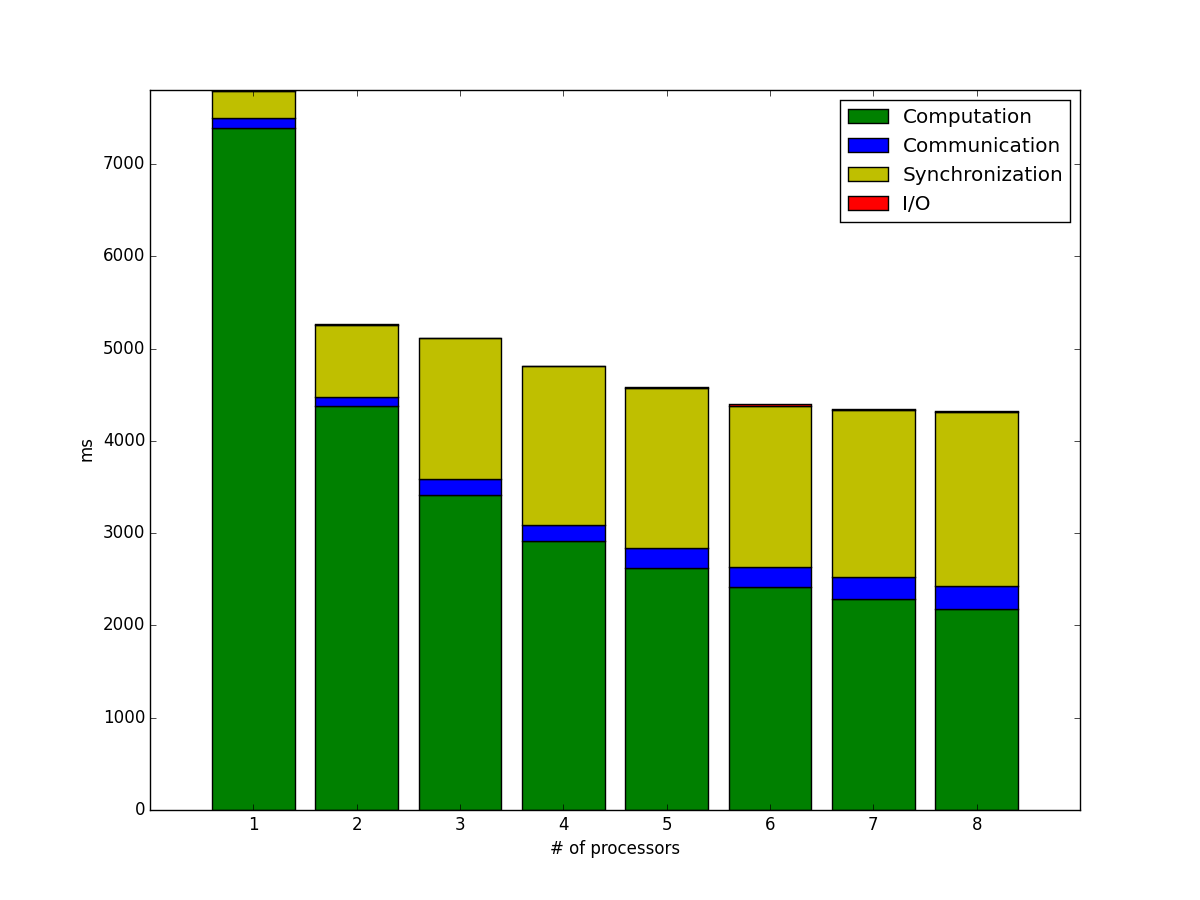
\includegraphics[scale=.4]{../run_report/basic/single-exec.png}
		\end{minipage}
		\hspace{4.5em}
		\begin{minipage}{.52\textwidth}
			\hspace{-3em}
			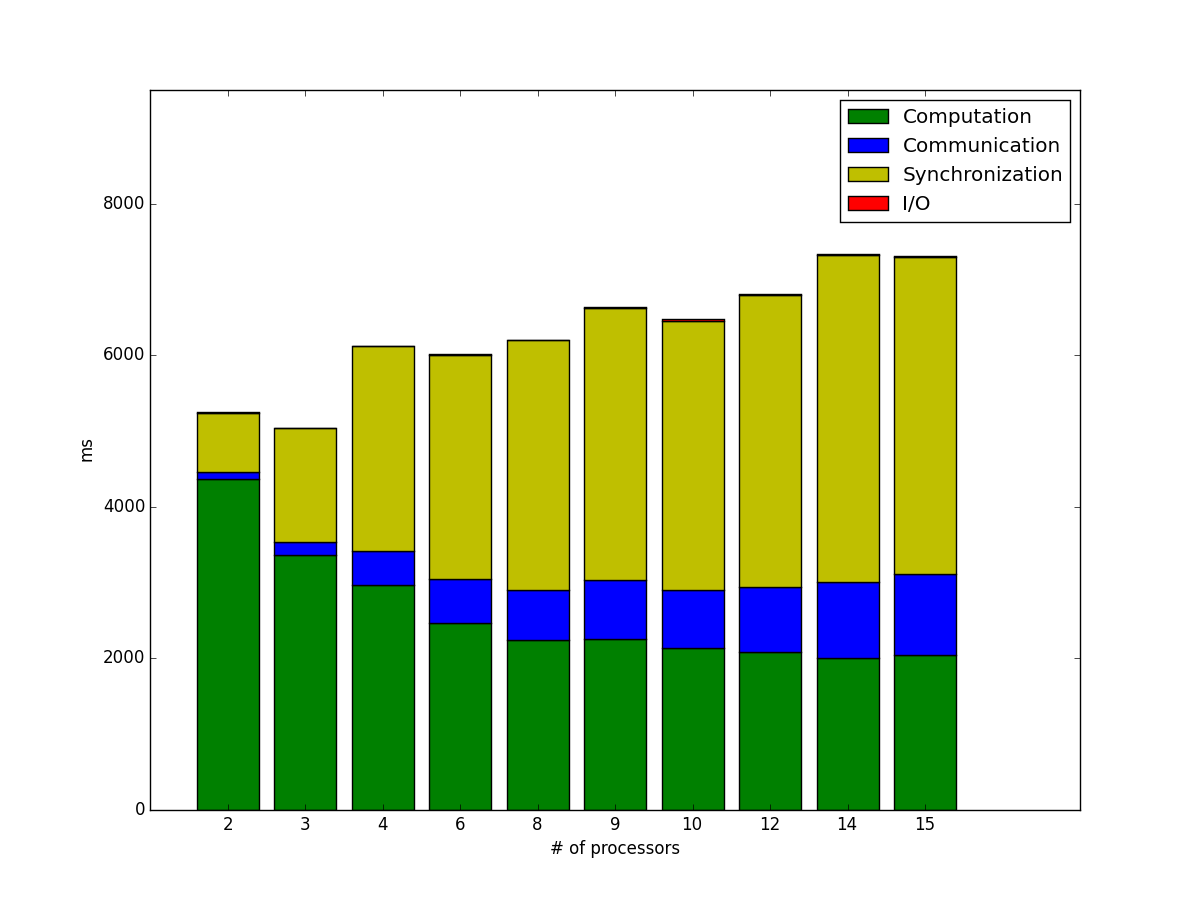
\includegraphics[scale=.4]{../run_report/basic/multiple-exec.png}
		\end{minipage}
	\end{figure}

	\newpage

	\item Advanced-bubble
	\begin{figure}[ht]
		\begin{minipage}{.45\textwidth}
			\hspace{-4.5em}
			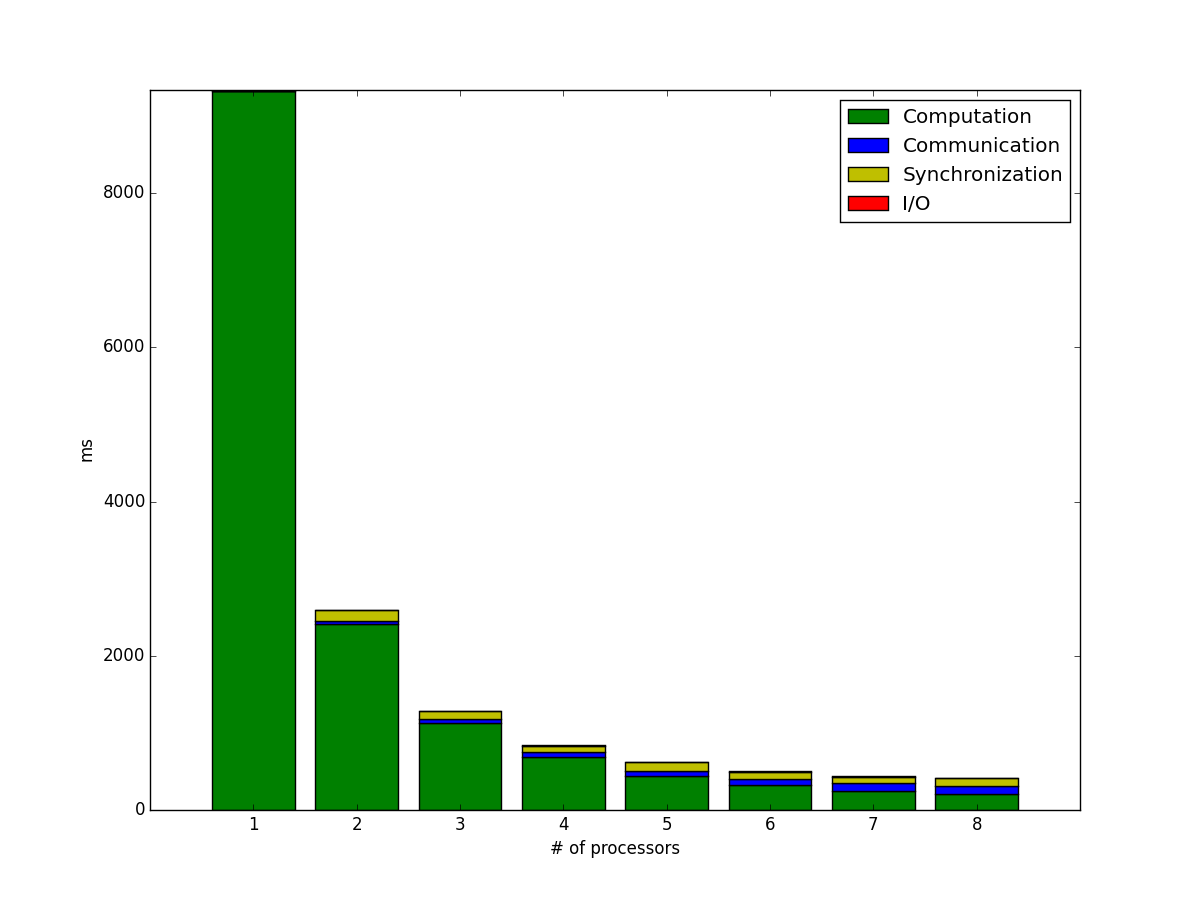
\includegraphics[scale=.4]{../run_report/advanced/bubble/single-exec.png}
		\end{minipage}
		\hspace{4.5em}
		\begin{minipage}{.52\textwidth}
			\hspace{-3em}
			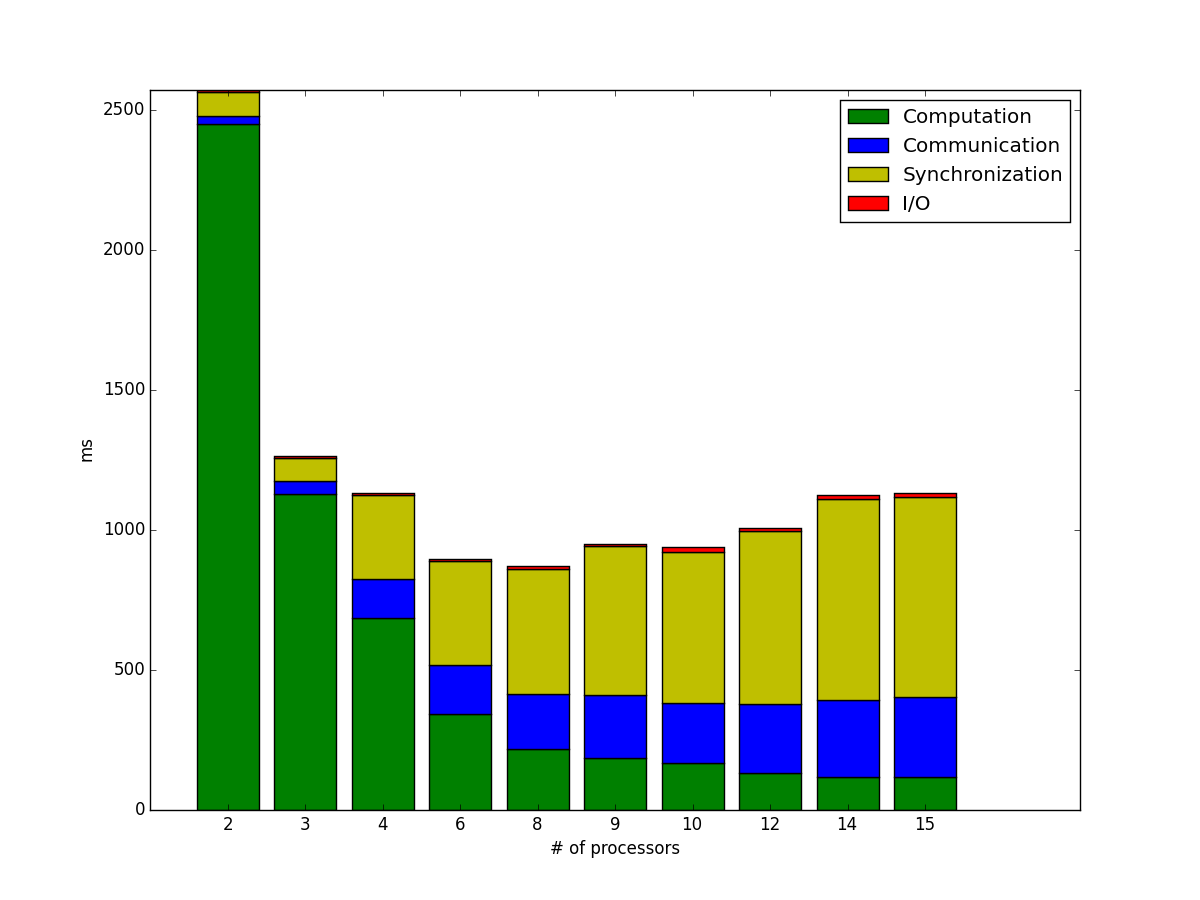
\includegraphics[scale=.4]{../run_report/advanced/bubble/multiple-exec.png}
		\end{minipage}
	\end{figure}

	\item Advanced-merge
	\begin{figure}[ht]
		\begin{minipage}{.45\textwidth}
			\hspace{-4.5em}
			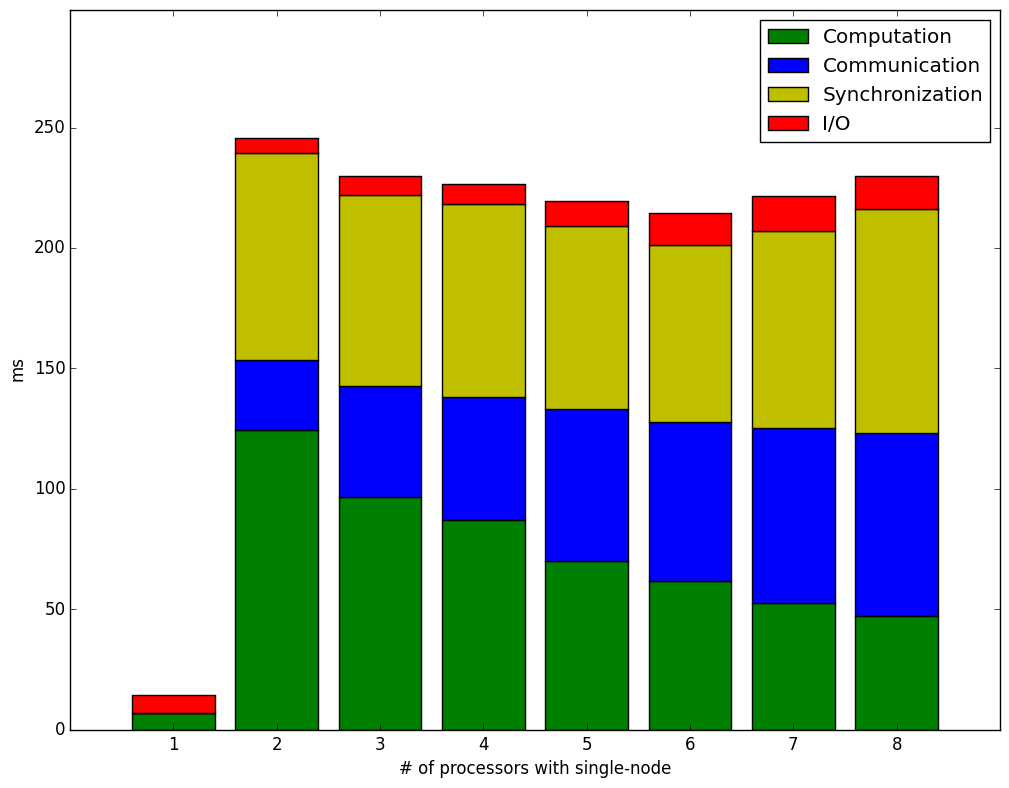
\includegraphics[scale=.4]{../run_report/advanced/merge/single-exec.png}
		\end{minipage}
		\hspace{4.5em}
		\begin{minipage}{.52\textwidth}
			\hspace{-3em}
			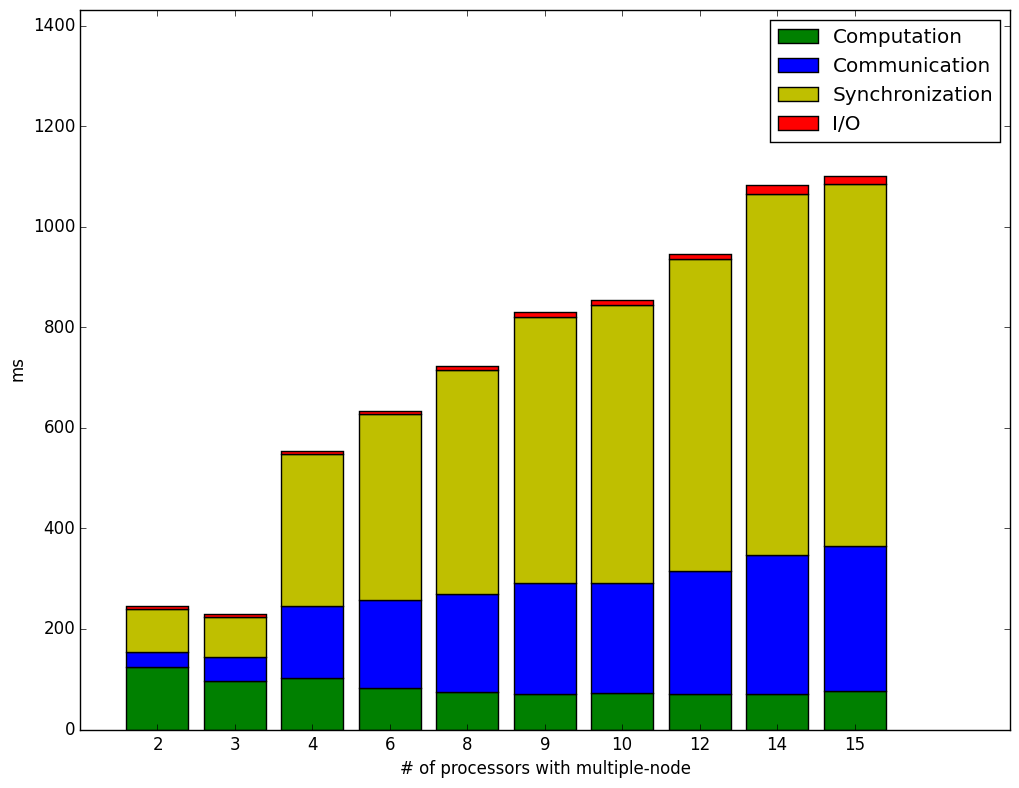
\includegraphics[scale=.4]{../run_report/advanced/merge/multiple-exec.png}
		\end{minipage}
	\end{figure}

	\newpage

	\item Speedup \& Overall execution
	\begin{flushleft}
		Execution time figure has been shown at right-hand side, it shows the performance of advanced version is superior to that of basic version.
	\end{flushleft}
	\begin{figure}[ht]
		\begin{minipage}{.49\textwidth}
			\hspace{-4.5em}
			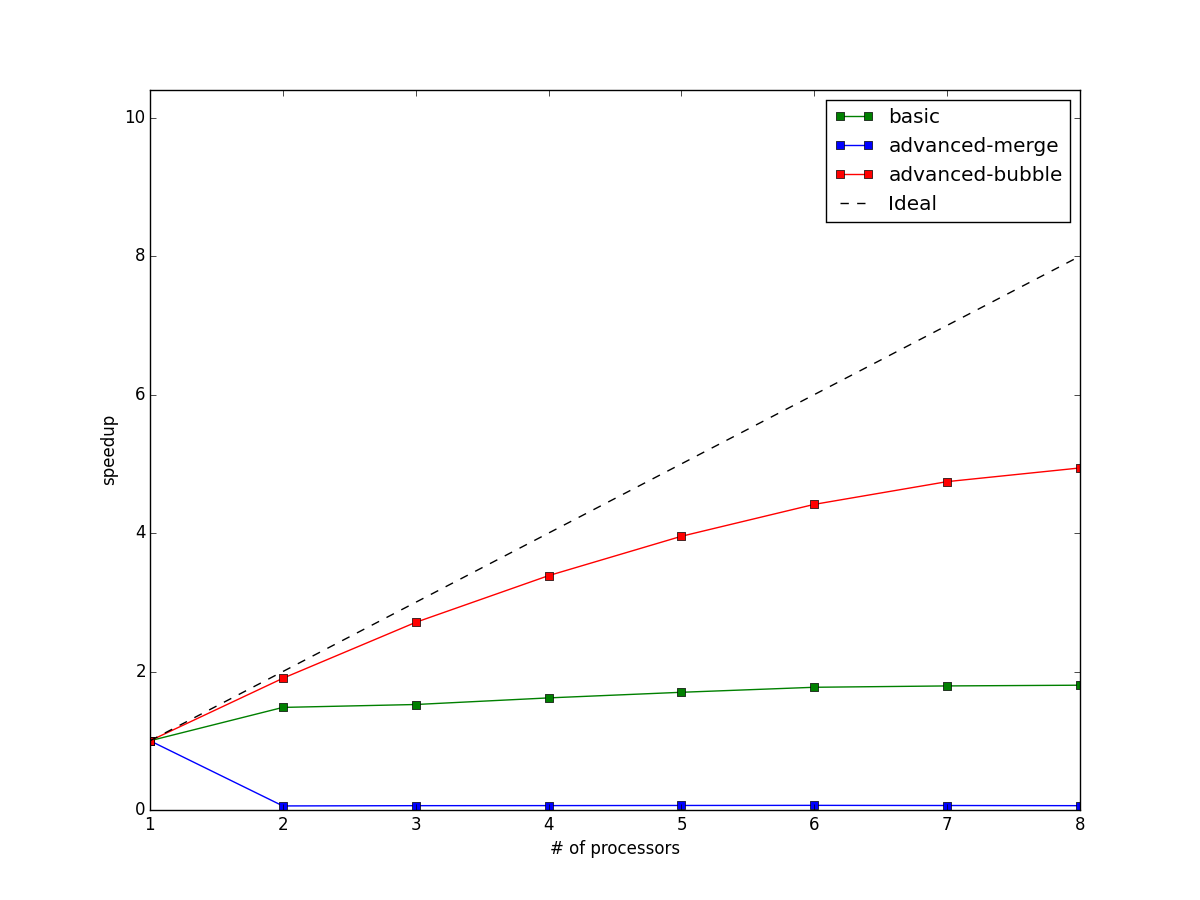
\includegraphics[scale=.4]{../run_report/speedup.png}
		\end{minipage}
		\hspace{3em}
		\begin{minipage}{.49\textwidth}
			\hspace{-3em}
			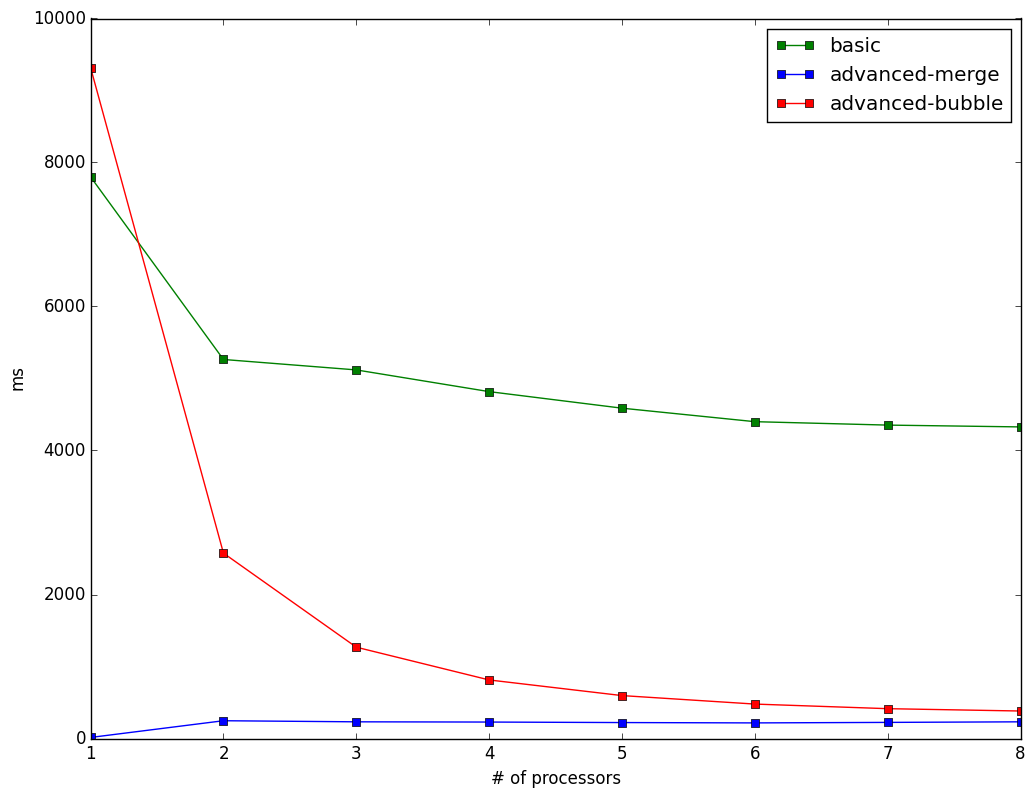
\includegraphics[scale=.4]{../run_report/overall_exec.png}
		\end{minipage}
	\end{figure}

	\item I/O Strategies
	\begin{SCfigure}[][h]
		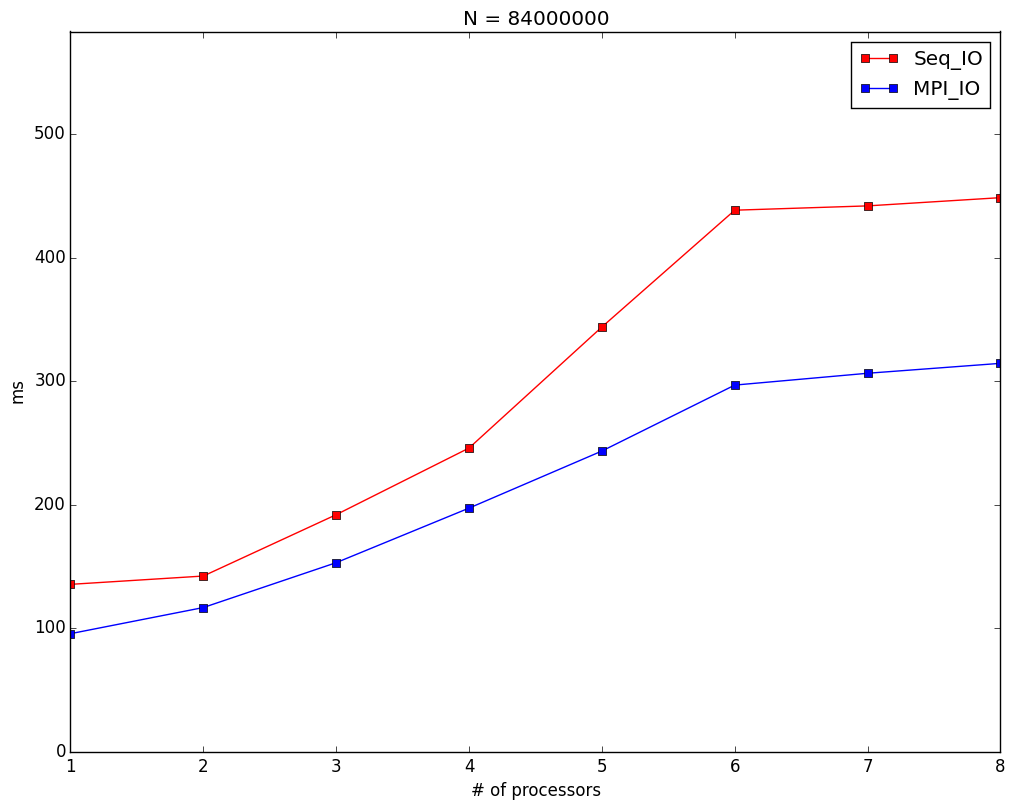
\includegraphics[scale=.45]{../run_report/io_diff.png}
		\caption{Execution time between different I/O.
		\newline Consumption time rises as the number of processors increases, and MPI\_IO is always faster than Seq\_IO}
	\end{SCfigure}
\end{itemize}

\newpage

\section*{Discussion}
\vspace{-20pt}
\noindent\makebox[\linewidth]{\rule{\textwidth}{0.4pt}}

\begin{enumerate}
	\item Work Balance
	\begin{flushleft}
		It requires less communication time with single node than with multiple node, and then it requires less synchronization time also. With different strategies:
	\end{flushleft}
	\begin{itemize}
		\item Basic
		\begin{flushleft}
			According to the consumption of synchronization, it shows the loading scheduling is not balanced. In each iteration, each processor should check all pairs it possesses and determine if the pair should be swapped. I think it is the main reason why the loading scheduling is not balanced because it is hard to presume each processor has same numbers of instructions at each iteration.
		\end{flushleft}
		\item Advanced
		\begin{flushleft}
			In advanced version, the data in each processor has been sorted before communication. The insertion operation consists of searching ($O(\log(N))$) and array moving ($O(N)$), it guarantees the task will be well-balanced because each processor keeps same size of numbers. In addition, merge sort is not suitable in this kind of strategy because the complexity will be significantly smaller when $p = 1$, and required execution time rises as $p$ increases.
		\end{flushleft}
	\end{itemize}

	\item Speedup Efficiency
	\begin{flushleft}
		According to the result, the performance of advanced-bubble is the best, and that of advanced-merge is the worst. The bad result of advanced-merge is because the time consumed in swapping stage is highly larger than pre-sorting and will dominate the overall execution time. After all, the result has verified that the efficiency is subject to how well the work is balanced.
	\end{flushleft}
\end{enumerate}

\end{CJK}
\end{document}